\documentclass[12pt]{article}

\usepackage{amsmath}
\usepackage{amssymb}
\usepackage{amsfonts}
\usepackage[style=iso]{datetime2}
\usepackage{graphicx}

\graphicspath{ {./Images/} }

\begin{titlepage}
\title{Calculus I: Review of Trigonometric Functions}
\author{The Melon Man}
\date{\today}
\end{titlepage}

\renewcommand{\thesection}{\Roman{section}}

\allowdisplaybreaks

\setlength{\parindent}{0pt}
\setlength{\parskip}{1em}

\begin{document}
\maketitle

\begin{figure}[h]
    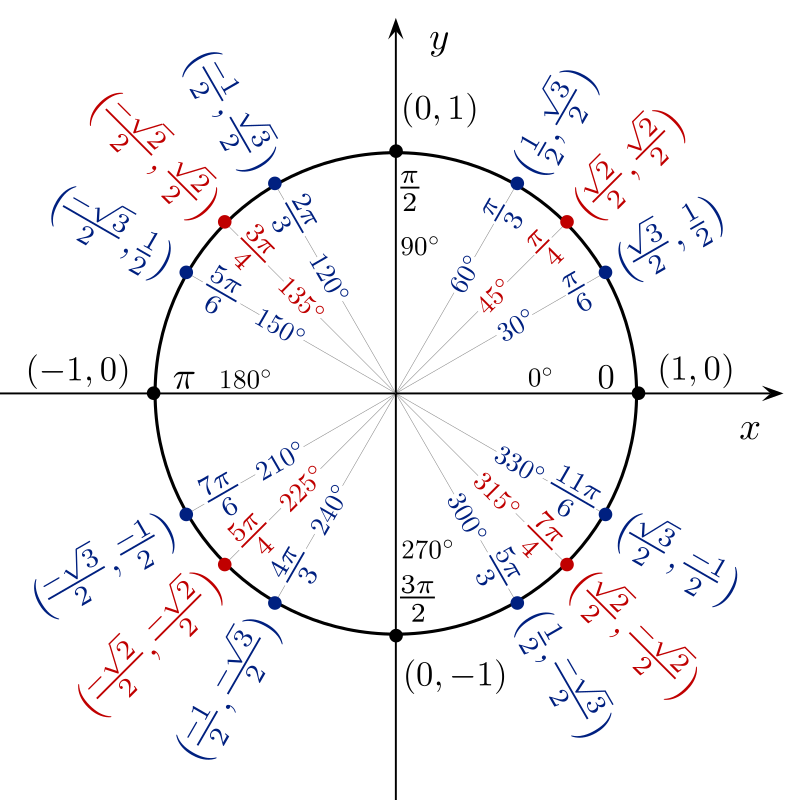
\includegraphics[width=10cm, height=10cm]{unit_circle.png}
    \centering
    \caption{The Unit Circle}
    \label{fig:fig1}
\end{figure}

Above is the unit circle.
It is important to be familiar with it as it is needed when looking at trig functions and equations.
The unit circle is important as we use it to define the trig functions.
The six trig functions may be defined in reference to the sides of a right-angled triangle, as follows:

\begin{align}
    \sin(\theta) & = \frac{O}{H} \\
    \cos(\theta) & = \frac{A}{H} \\
    \tan(\theta) & = \frac{O}{A} \\
    \csc(\theta) & = \frac{H}{O} \\
    \sec(\theta) & = \frac{H}{A} \\
    \cot(\theta) & = \frac{A}{O}
\end{align}

where O is the opposite side of a right triangle in reference to an angle, A is the adjacent side and H is the hypotenuse or diagonal side of the triangle.

We may define the unit circle as a circle of radius $1$ centered at the origin.
Inside, we may have a right triangle with some angle $\theta$.
By defining our trig functions in reference to this, we may notice that the sine of the angle will be $y$ position of the triangle touching the circumference of the circle, due to the circle having radius $1$
Similarly, the cosine of the angle represents the $x$ position.
The other trig functions may be defined in reference to those two.
This fact may be noticed as all three sides of the triangle are covered by the sine and cosine functions.
Therefore, the other trig functions, which are also ratios of sides, may be defined in reference to the sine and cosine functions.

Something else relating to trig functions that is quite important in a calc course is radians.
Radians are another way of representing an angle, as opposed to degrees.
In calculus, we use radians as they are more convenient to work with.
They are defined with reference to a circle and its radius.
One radian is defined as the angle subtended by an arc of length equal to the radius of the circle.
Therefore, the circumference of a circle is $2\pi$ radians.
We could then translate from radians to degrees by using the fact that $360$ degrees is equal to $2\pi$ radians.
This means that $180$ degrees is equal to $\pi$ radians and $90$ degrees is equal to $\frac{\pi}{2}$ radians.
You should be able to convert between radians and degrees, though we will not make particular use of degrees in this course.

You should be able to find the exact values of trig functions with the unit circle.
Notice the symmetries present and the fact that the values of the trig functions will be the same at some interval.
This makes them periodic.
Both the sine and cosine functions are periodic with period $2\pi$, meaning that the unit circle can be used for any angle.
For instance, the angle $\frac{7\pi}{3}$ shows one full rotation around the circle and then another $\frac{\pi}{3}$ radians.
While the unit circle may look complicated, you only need to remember the first quadrant.
The other quadrants are just reflections of the first quadrant so you can use a bit of geometry to figure the rest out.

With reference to the unit circle, give the exact values of the following:

\begin{enumerate}
    \item $\displaystyle \cos \left( {\frac{{5\pi }}{6}} \right)$
    \item $\displaystyle \sin \left( { - \frac{{4\pi }}{3}} \right)$
    \item $\displaystyle \sin \left( {\frac{{7\pi }}{4}} \right)$
    \item $\displaystyle \cos \left( { - \frac{{2\pi }}{3}} \right)$
    \item $\displaystyle \tan \left( {\frac{{3\pi }}{4}} \right)$
    \item $\displaystyle \sec \left( { - \frac{{11\pi }}{6}} \right)$
    \item $\displaystyle \cos \left( {\frac{{8\pi }}{3}} \right)$
    \item $\displaystyle \tan \left( { - \frac{\pi }{3}} \right)$
    \item $\displaystyle \tan \left( {\frac{{15\pi }}{4}} \right)$
    \item $\displaystyle \sin \left( { - \frac{{11\pi }}{3}} \right)$
    \item $\displaystyle \sec \left( {\frac{{29\pi }}{4}} \right)$
\end{enumerate}

The answers are as follows:

\begin{enumerate}
    \item $\displaystyle -\frac{\sqrt{3}}{2}$
    \item $\displaystyle \frac{\sqrt{3}}{2}$
    \item $\displaystyle -\frac{\sqrt{2}}{2}$
    \item $\displaystyle -\frac{1}{2}$
    \item $\displaystyle -1$
    \item $\displaystyle \frac{2}{\sqrt{3}}$
    \item $\displaystyle -\frac{1}{2}$
    \item $\displaystyle -\sqrt{3}$
    \item $\displaystyle -1$
    \item $\displaystyle \frac{\sqrt{3}}{2}$
    \item $\displaystyle -\sqrt{2}$
\end{enumerate}

This is not all the trig required for calculus, but it is most of the important stuff.
There are some important identities and formulae that you should know, but those will be mentioned when they are needed.
Really, the ability to evaluate the sine and cosine function at some angles with the unit circle is the most important thing.
Most of the other stuff, even the identities and other trig functions, can be derived from the unit circle and algebraic manipulation.

\end{document}